\documentclass[12pt]{article}
\usepackage{graphicx}
\usepackage{gensymb}
\usepackage[none]{hyphenat}
\usepackage{graphicx}
\usepackage{listings}
\usepackage[english]{babel}
\usepackage{graphicx}
\usepackage{caption}
\usepackage{hyperref}
\usepackage{booktabs}
\usepackage{array}
\usepackage{amsmath}
\usepackage{listings}
\graphicspath {./sdcard/fwc/}
\lstset{
        frame=single'
	breaklines=true
	}
\newcommand{\mydet}[1]{\ensuremath{\begin{vmatrix}#1\end{vmatrix}}}
\providecommand{\brak}[1]{\ensuremath{\left(#1\right)}}
\providecommand{\norm}[1]{\left\lVert#1\right\rVert}
\newcommand{\solution}{\noindent \textbf{Solution: }}
\newcommand{\myvec}[1]{\ensuremath{\begin{pmatrix}#1\end{pmatrix}}}
\let\vec\mathbf	

\begin{document}
\begin{center}
\textbf\large{CHAPTER - 9  \\  TRIANGLES}
\section*{EXERCISE - 9.4}
\end{center}

\begin{enumerate}

\item A point $\vec{E} $ is taken on the side $\vec{BC} $ of a parallelogram $\vec{ABCD} $.$\vec{AE}$ and  $\vec{DC}$ are produced to meet at $\vec{F}$.Prove that  ar $\vec{(ADF)}$ = ar $\vec{(ABFC)}$.
\item The diagonals of a parallelogram $\vec{ABCD}$ intersect at a point $\vec{O}$.Through $\vec{O}$,a line is drawn to intersect $\vec{AD}$ at $\vec{P}$ and $\vec{BC}$ at $\vec{Q}$.Show that $\vec{PQ}$ divides the parallelogram into two parts of equal area.
\item The medians $\vec{BE}$ and $\vec{CF}$ of a triangle $\vec{ABC}$ intersect at $\vec{G}$.Prove that the area of $ \triangle\vec{GBC} $= area of the quadrilateral $\vec{AFGE}$.	
\item In Fig.\ref{fig:9.24},$\vec{CD} \parallel \vec{AE} $ and $ \vec{CY} \parallel \vec{BA} $.Prove that ar $\vec{(CBX)}$ = ar $\vec{(AXY)}$
\begin{figure}[h]
	\centering
	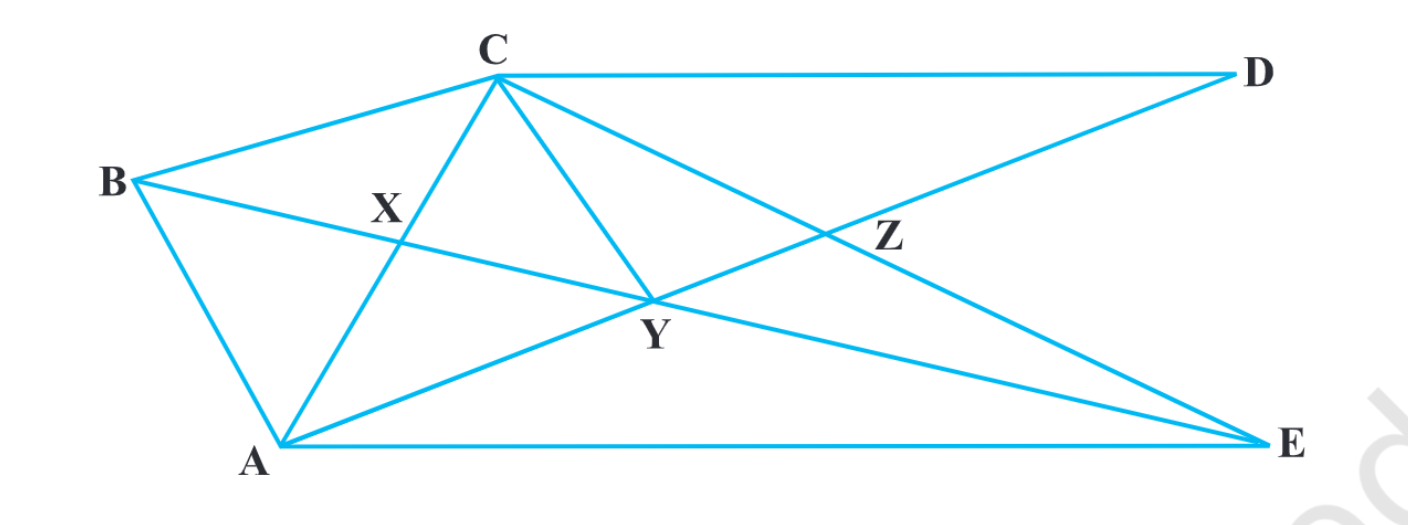
\includegraphics[width=9cm]{Figs/Fig9.24.png}
	\caption{}
	\label{fig:9.24}
\end{figure}
\item $\vec{ABCD}$ is a trapezium in which $\vec{AB} \parallel \vec{DC} $,$\vec{DC} = 30 cm $  and \\ $\vec{AB} = 50 cm $.If $\vec{X}$ and $\vec{Y}$ are,respectively the mid-points of $\vec{AD}$ and $\vec{BC}$,prove that  ar $\vec{(DCYX)} = \frac{7}{9}$ ar $\vec{(XYBA)} $.
\item  In $ \triangle\vec{ABC} $,if $\vec{L}$ and $\vec{M}$ are the points on $\vec{AB}$ and $\vec{AC}$,respectively such that $ \vec{LM} \parallel \vec{BC} $.Prove that ar $\vec{(LOB)}$ = ar $\vec{(MOC)}$.
\newpage
\item In Fig.\ref{fig:9.25},$\vec{ABCDE}$ is any pentagon.$\vec{BP}$ drawn parallel to $\vec{AC}$ meets $\vec{DC}$ produced at $\vec{P}$ and $\vec{EQ}$ drawn parallel to $\vec{AD}$ meets $\vec{CD}$ produced at $\vec{Q}$.Prove that ar $\vec{(ABCDE)}$ = ar $\vec{(APQ)}$.
\begin{figure}[h]
	\centering
	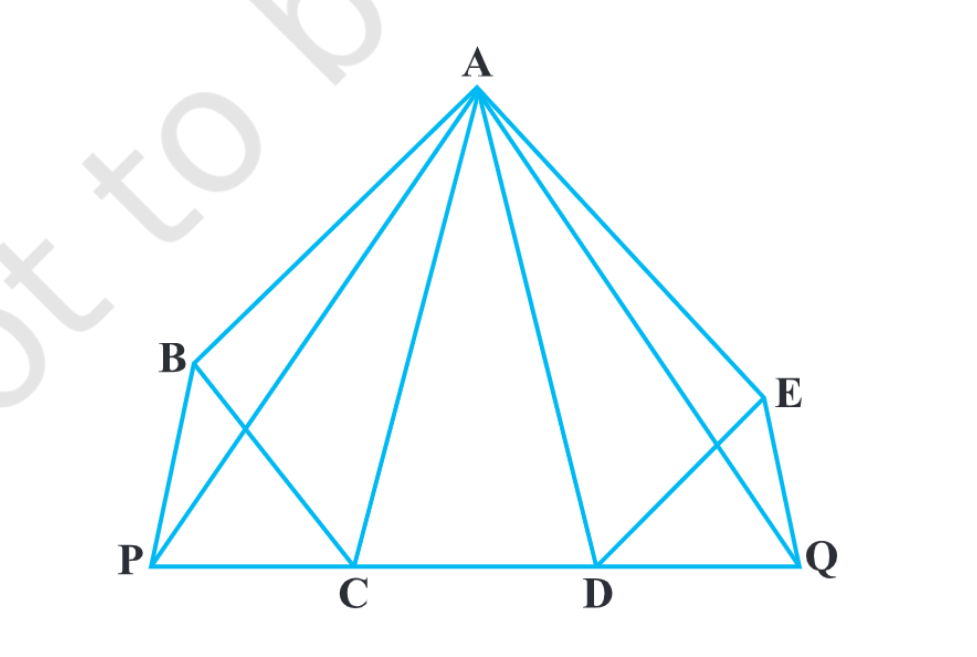
\includegraphics[width=9cm]{Figs/Fig9.25.png}
	\caption{}
	\label{fig:9.25}
\end{figure}
\item If the medians of a $ \triangle\vec{ABC} $ intersect at $\vec{G}$,show that  \\ ar $\vec{(AGB)}$ = ar $\vec{(AGC)}$ = ar $\vec{(BGC)}$ = $\frac{1}{3}$ ar $\vec{(ABC)}  $.
\item In Fig.\ref{fig:9.26},$\vec{X}$ and $\vec{Y}$ are the mid-points of $\vec{AC}$ and $\vec{AB}$ respectively,$\vec{QP} \parallel \vec{BC} $ and $\vec{CYQ}$ and $\vec{BXP}$ are straight lines.Prove that \\ ar $\vec{(ABP)}$ = ar $\vec{(ACQ)}$.
\begin{figure}[h]
	\centering
	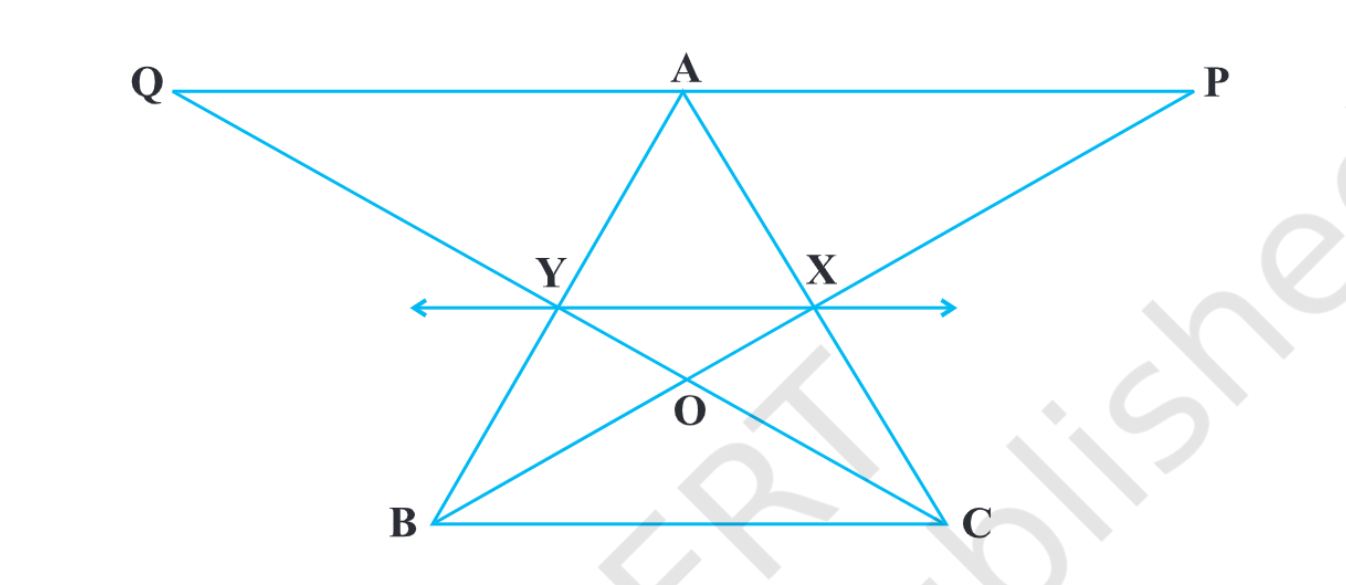
\includegraphics[width=9cm]{Figs/Fig9.26.png}
	\caption{}
	\label{fig:9.26}
\end{figure}
\newpage
\item In Fig.\ref{fig:9.27},$\vec{ABCD}$ and $\vec{AEFD}$ are two parallelograms.Prove that \\ ar $\vec{(PEA)}$ = ar $\vec{(QFD)}$  [Hint:Join PD].
\begin{figure}[h]
	\centering
	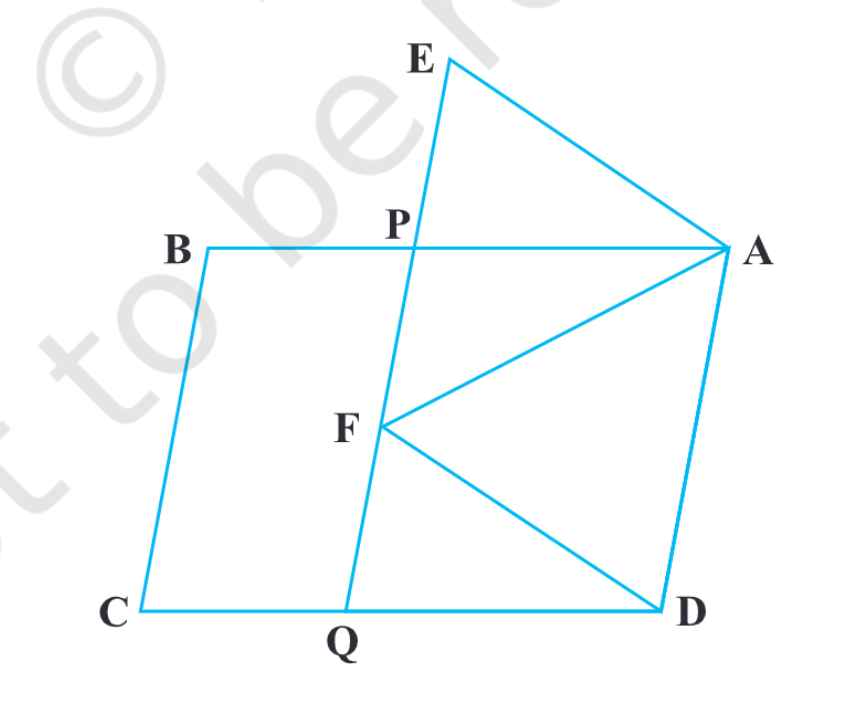
\includegraphics[width=9cm]{Figs/Fig9.27.png}
	\caption{}
	\label{fig:9.27}
\end{figure}
\end{enumerate}
\end{document}


	
		
	
